%%%%%%%%%%%%%%%%%%%%%%%%%%%%%%%%%%%%%%%%%%%%%%%%%%%%%%%%%%%%%%%%%
%2345678901234567890123456789012345678901234567890123456789012345
%        1         2         3         4         5         6     
\chapter{Quadratic ICR optimization problem}
\label{cha:Quadratic}

An early control method for MIMO systems is the linear quadratic regulator (LQR) for an unconstrained objective function for states and inputs.
Model predictive control (MPC) is an advanced control approach evolved from LQR.
\cite{Morari.1999} gives amongst other things a survey on the history of MPC.

\cref{sec:mpc_glance} shows the basic principles of MPC. 
In \cref{sec:processmodel} the derivation of process models and their requirements for MPC are presented.
\cref{sec:prediction} shows how system evolution can be described only in dependence of the input trajectory and the current states.
The objective, its effect on the control and the consideration of constraints is explained in \cref{sec:objective}.

%%%%%%%%%%%%%%%%%%%%%%%%%%%%%%%%%%%%%%%%%%%%%%%%%%%%%%%%%%%%%%%%%%%%%%%%%%%%%%%%%%%%%%%%%%%%%%%%%%%%%%%%%%%%%%%%%%%%%%%%%%%%%%%%%%%%%%%%%%%%%%%%%%%%%%%%%%%%%%%%%%%%%%%%%%%%%%%%%%%%%%%%%%%%%%%%

\section{MPC at a glance}
\label{sec:mpc_glance}

MPC uses knowledge about a complex and often multi-variable system's properties to compute an input trajectory that is optimal with respect to an arbitrary defined objective function while considering the constraints.
MPC schemes can be linear and nonlinear.
For an further introduction to MPC \cite{Rawlings.2009} is proposed. For theory, design and applications of nonlinear MPC  \cite{Grune.2011} and \cite{Grancharova.2012b} are recommended.

\begin{figure}[t]
\begin{center}
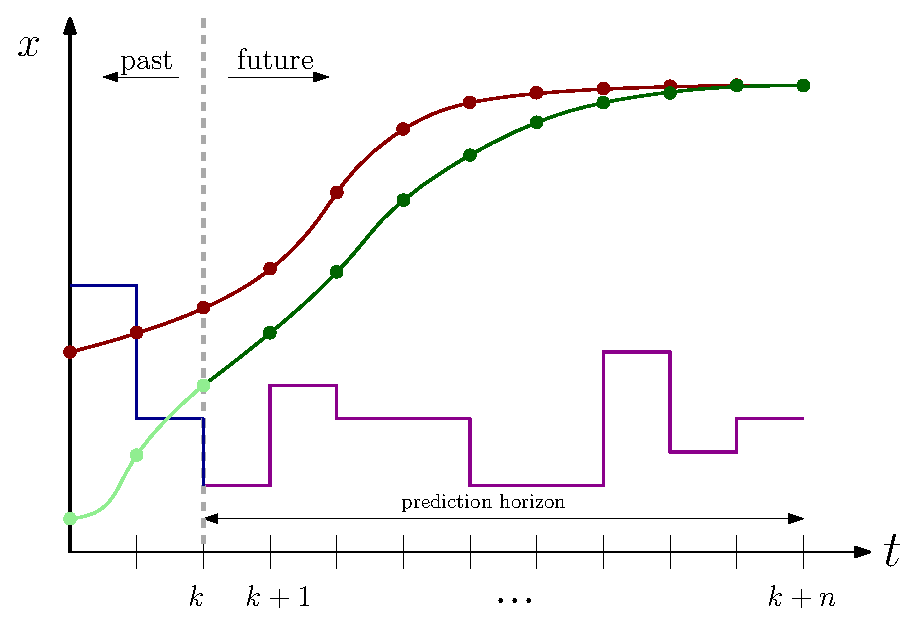
\includegraphics[width=\textwidth]{../Figures/MPC_trajectory.eps}
\caption{Example of a time-discrete MPC scheme: red - reference trajectory, light green - measured state trajectory, dark green - predicted state trajectory, violet - optimal control trajectory}
\label{fig:controller}
\end{center}
\end{figure}

Model predictive control has its roots in optimal control. Basically, a model is used to forecast the system's future behaviour. This knowledge is used to find an optimal trajectory of control inputs. For this computations, MPC needs a process model and an optimization algorithm.
MPC consists of four repeating steps::
\begin{enumerate}
	\item Obtain the current state
	\item Predict the system evolution
	\item Calculate optimal input trajectory
	\item Apply optimal input
\end{enumerate}

\cref{fig:controller} depicts one step of the MPC algorithm. The objective is that the green line, the system's real state, is as close as possible to the red line, the reference trajectory. Therefore the violet line is the optimal control trajectory of future inputs.

%%%%%%%%%%%%%%%%%%%%%%%%%%%%%%%%%%%%%%%%%%%%%%%%%%%%%%%%%%%%%%%%%%%%%%%%%%%%%%%%%%%%%%%%%%%%%%%%%%%%%%%%%%%%%%%%%%%%%%%%%%%%%%%%%%%%%%%%%%%%%%%%%%%%%%%%%%%%%%%%%%%%%%%%%%%%%%%%%%%%%%%%%%%%%%%%

\section{Process model}
\label{sec:processmodel}

To guarantee a good performance of a MPC, the quality of the process model which is used for the predictions is crucial.
The model has to capture the major dynamics of the real controlled system otherwise the predicted states may deviate heavily from the real states.
Thus, the computed inputs may lead to constraint violations which render the control task infeasible.
To derive a process model, two general approaches can be considered.

The first one is first-principles modelling where the model is derived from physical laws.
The advantage of this method is that the parameters and their values have a meaning and the relations between the variables can be easily understood.
But it demands much knowledge in the specific field of application.

The second approach is system identification which can be generally divided into two groups.
In case of grey box system identification known relations and parameters are modelled while unknown ones are estimated via optimization with training data.
When black box system identification is applied, a strictly mathematical model with a certain amount of parameters is used, for example a neuronal network or a polynomial.

For all cases described above the obtained models have to be verified for different scenarios by comparing the real system with the process model.
The quality of the process model has to be optimized until it meets the requirements for a prediction model.
For more information about system identification see \cite{Isermann.2011} and \cite{Ljung.2012}.

The augmented MPC scheme presented in \cref{cha:implementation} relies on a linear continuous model:
\begin{equation}\label{eq:linss_cont}
\dot{\mathbf{x}}(t) = A\mathbf{x}(t)+B\mathbf{u}(t),
\end{equation}
where $\mathbf{x}(t)$ are states and $\mathbf{u}(t)$ are the inputs at time $t$.

However, since for solving the optimal control problem the continuous model is fully discretized at every time step $t_s$ using collocation our example system will be a linear discrete-time one described by:
\begin{equation}\label{eq:linss}
\mathbf{x}_{k+1}=A_{dis}\mathbf{x}_k+B_{dis}\mathbf{u}_k,
\end{equation}
where $\mathbf{x}_k$ are the states and $\mathbf{u}_k$ are the inputs at time step $k$.

%%%%%%%%%%%%%%%%%%%%%%%%%%%%%%%%%%%%%%%%%%%%%%%%%%%%%%%%%%%%%%%%%%%%%%%%%%%%%%%%%%%%%%%%%%%%%%%%%%%%%%%%%%%%%%%%%%%%%%%%%%%%%%%%%%%%%%%%%%%%%%%%%%%%%%%%%%%%%%%%%%%%%%%%%%%

\section{Prediction}
\label{sec:prediction}

If we want to predict the systems behaviour further than one step into the future, we have a function that is depending on future states.
In case of a prediction horizon of two time steps we can insert \eqref{eq:linss} in the first line of \eqref{eq:linpred2}.
\begin{align}\label{eq:linpred2}
\begin{split}
\mathbf{x}_{k+2} &= A_{dis} \mathbf{x}_{k+1} + B_{dis} \mathbf{u}_{k+1}, \\
                 &= A_{dis} \left(  A_{dis} \mathbf{x}_k + B_{dis} \mathbf{u}_k \right) + B_{dis} \mathbf{u}_{k+1}, \\
                 &= A_{dis}^2 \mathbf{x}_k + A_{dis} B_{dis} \mathbf{u}_k + B_{dis} \mathbf{u}_{k+1}.
\end{split}
\end{align}
Because the current state $\mathbf{x}_k$ and the current input $\mathbf{u}_k$ are known, $\mathbf{x}_{k+2}$ is only depending on $\mathbf{u}(T_s)$.
The same applies for predicting the state for all future time steps.
For the prediction of the states of the $n$-th future step at time step $k$ we get:
\begin{align}\label{eq:linpredn}
\begin{split}
\mathbf{x}_{k+n}&=A_{dis}^n\mathbf{x}_k+A_{dis}^{n-1}B_{dis}\mathbf{u}_k+\ldots\\
                &+A_{dis}B_{dis}\mathbf{u}_{k+n-2}+B_{dis}\mathbf{u}_{k+n-1}.
\end{split}
\end{align}
Thus, the future states are only a function of the current state $\mathbf{x}_k$ and the future inputs $\mathbf{u}_{k+i}$ which build the input trajectory.

%%%%%%%%%%%%%%%%%%%%%%%%%%%%%%%%%%%%%%%%%%%%%%%%%%%%%%%%%%%%%%%%%%%%%%%%%%%%%%%%%%%%%%%%%%%%%%%%%%%%%%%%%%%%%%%%%%%%%%%%%%%%%%%%%%%%%%%%%%%%%%%%%%%%%%%%%%%%%%%%%%%%%

\section{Objective function}
\label{sec:objective}

MPC is an optimal control approach with respect to the objective function.
The objective function describes the target of the control mathematically.
An example of a quadratic objective for the discrete-time state-space-model \eqref{eq:linss} is
\begin{equation}\label{eq:quadratic_cost}
J_{dis}(\mathbf{x},\mathbf{u}) = \sum_{k=1}^{n} (\mathbf{r}_k-\mathbf{x}_k)^TQ(\mathbf{r}_k-\mathbf{x}_k)+\mathbf{u}_k^TR\mathbf{u}_k,
\end{equation}
where $\mathbf{r}_k$ is the discrete reference trajectory, $n$ is the prediction horizon, $Q$ is the weighting matrix for states and $R$ is the weighting matrix for the inputs.
Large positive values in $Q$ result in a focus on sticking close to the reference trajectory while large positive values in $R$ enforce the minimization of used actuation energy.
To find the optimal input trajectory, the objective hast to be minimized while considering the constraints.

The resulting optimal control problem is described by:
\begin{subequations} \label{eq:description_conventional_mpc}
\begin{align}
\min \, J_{dis}(\mathbf{x},\mathbf{u})
\end{align}
subject to:
\begin{align}
\mathbf{x}_{k+1} = A\mathbf{x}_k+B\mathbf{u}_k,\\
\mathbf{x}_i \in \mathcal{X}, \mathbf{u}_i  \in \mathcal{U},\\
x_0 = x_{\text{init}},
\end{align}
\end{subequations}
where $\mathcal{X}$ and $\mathcal{U}$ are the compact and bounded spaces for feasible states and feasible inputs.

The state constraints are often implemented as box constraints.
Thus, they define the allowed maximum deviation from the reference trajectory.
The input constraints often describe the physical limits of the actuators.
As well the state constraints as the input constraints can be defined as soft and hard constraints.
The violation of hard constraints lead directly to an infeasible optimization problem, whereas the violation of soft constraints add a penalty term to the objective:
\begin{equation}\label{eq:soft}
J_{dis,soft}(\mathbf{x},\mathbf{u}) = J(\mathbf{x},\mathbf{u}) + \delta \sum_{k=1}^{n} \mathbf{v}_k,
\end{equation}
where $\delta$ is the weight of the penalty and $\mathbf{v}_k$ is the absolute value of the violation at time step $k$.

\eqref{eq:quadratic_cost} is a conventional objective function.
However, there are many approaches to design a economic objective function for minimizing the costs or maximizing the profit. 
A maximization problem can be easily transformed to a minimization problem by:
\begin{equation}\label{eq:minmaxJ}
\max \, J(\mathbf{x},\mathbf{u}) = \min \, -J(\mathbf{x},\mathbf{u}).
\end{equation}
In \cref{cha:economic} an approach to minimize the cost of operating a greenhouse is presented.

Since the models used in the following chapters are continuous the description of a continuous optimal control for \eqref{eq:linss_cont} given by:
%\begin{equation}\label{eq:description_conventional_mpc_cont}
%\begin{split}
%\min \, J_{cont}(\mathbf{x}(t),\mathbf{u}(t)) \quad s.t.\\
%\dot{\mathbf{x}}(t) = A\mathbf{x}(t)+B\mathbf{u}(t),\\
%\mathbf{x}(t) \in \mathcal{X}, \mathbf{u}(t)  \in \mathcal{U},\\
%\end{split}
%\end{equation}
\begin{subequations} \label{eq:description_conventional_mpc_cont}
\begin{align}
\min \, J_{cont}(\mathbf{x}(t),\mathbf{u}(t)) 
\end{align}
subject to:
\begin{align}
\dot{\mathbf{x}}(t) = A\mathbf{x}(t)+B\mathbf{u}(t),\\
\mathbf{x}(t) \in \mathcal{X}, \mathbf{u}(t)  \in \mathcal{U} \\
x_0 = x_{\text{init}},
\end{align}
\end{subequations}
where the objective function for the continuous case is described by:
\begin{equation}\label{eq:quadratic_cost_cont}
J_{cont}(\mathbf{x}(t),\mathbf{u}(t)) = \int_{0}^{t_f} \! (\mathbf{r}(t)-\mathbf{x}(t))^TQ(\mathbf{r}(t)-\mathbf{x}(t))+\mathbf{u}(t)^TR\mathbf{u}(t)\mathrm{d}t,
\end{equation}
where $\mathbf{r}(t)$ is the continuous reference trajectory and ${t_f}$ is the prediction horizon.

The relation between the prediction horizon of the continuous and the discrete-time is:
\begin{equation}\label{eq:rel_cont_dis}
t_f = n \cdot t_s.
\end{equation}
\par\medskip

In this chapter the model predictive control approach was explained.
Moreover, insight was given about prediction models, 
Thus, the first theoretical foundation of the expanded linear model predictive control scheme derived in \cref{cha:implementation} was presented.
In the following chapter GPs are presented which build the second theoretical foundation.

